\newpage \chapter{\textbf{Model WCS With Execution Graphs}}

\section{Demand Vector}

Analyzing the sequence diagram, component and deployment diagram we have obtained this demand vector which represents virtual resources related to our architecture:

\begin{longtable}{|p{6cm}|p{9cm}|}

\hline
\textbf{Wired Connection Request} & Estimated consumption of the 											request to the Wired Connection \\

\hline
\textbf{Wireless Connection Request} & Estimated consumption of the 										   request to the Wireless 												   Connection \\

\hline
\textbf{Internet Connection Request} & Estimated consumption of the 										   request to the Internet 												   Connection \\

\hline
\textbf{Database Request} & Estimated consumption of the request to 								the Database \\ 

\hline
\textbf{Control Center Server CPU} & Estimated consumption of the 											 request to the Control Center 											 Server CPU\\

\hline
\textbf{Water Company Server CPU} & Estimated consumption of the 											request to theWater Company Server										CPU\\

\hline
\textbf{Purification System Pomezia CPU} & Estimated consumption of 											   the request to the 													   Purification System Pomezia 										   CPU\\


\hline
\textbf{Seaweed Picking Inland Control Unit CPU} & Estimated 															   consumption of 											   			   the request to the 													   Seaweed Picking 														   Inland Control Unit 												   CPU\\

\hline
\textbf{Seaweed Picking Outgoing Control Unit CPU} & Estimated 															   consumption of 											   			   the request to the 													   Seaweed Picking 														   Outgoing Control 													   Unit CPU\\

\hline
\textbf{Seaweed Picking Outgoings Sample Request} & Estimated 															   consumption of 											   			   the request to the 													   Seaweed Picking 														   Outgoing Sample \\

\hline
\textbf{Seaweed Picking Inlands Sample Request} & Estimated 															  consumption of 											   			  the request to the 													  Seaweed Picking 														  Inlands Sample \\
\hline
\end{longtable}

\newpage

The Execution Graphs obtained are:

\begin{itemize}
\item Sampling Water activated by Sample Supervisor:
	\bigskip
	\bigskip
	\begin{center}
 	 \makebox[\textwidth]{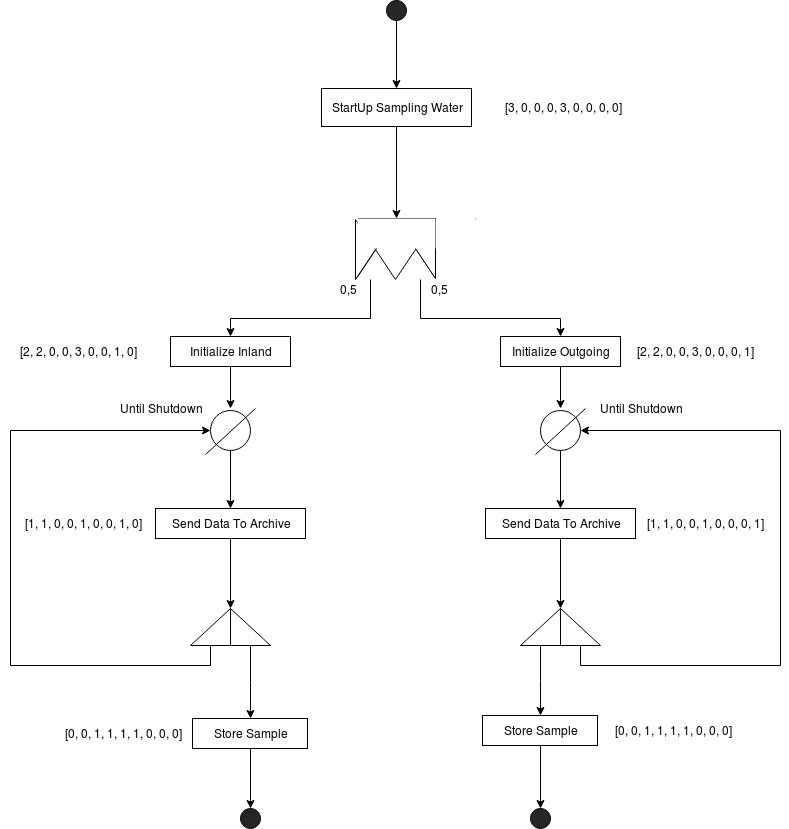
\includegraphics[width=\textwidth]				{EGUC1StartUpSamplingWater.jpg}}
	\end{center}
	\bigskip
	\captionof{figure}{EG UC1 StartUp Sampling Water}
\newpage
\item Check Water Quality activated by Quality Control Supervisor:
	\bigskip
	\bigskip
	\bigskip
	\bigskip
	\begin{center}
 	 \makebox[\textwidth]{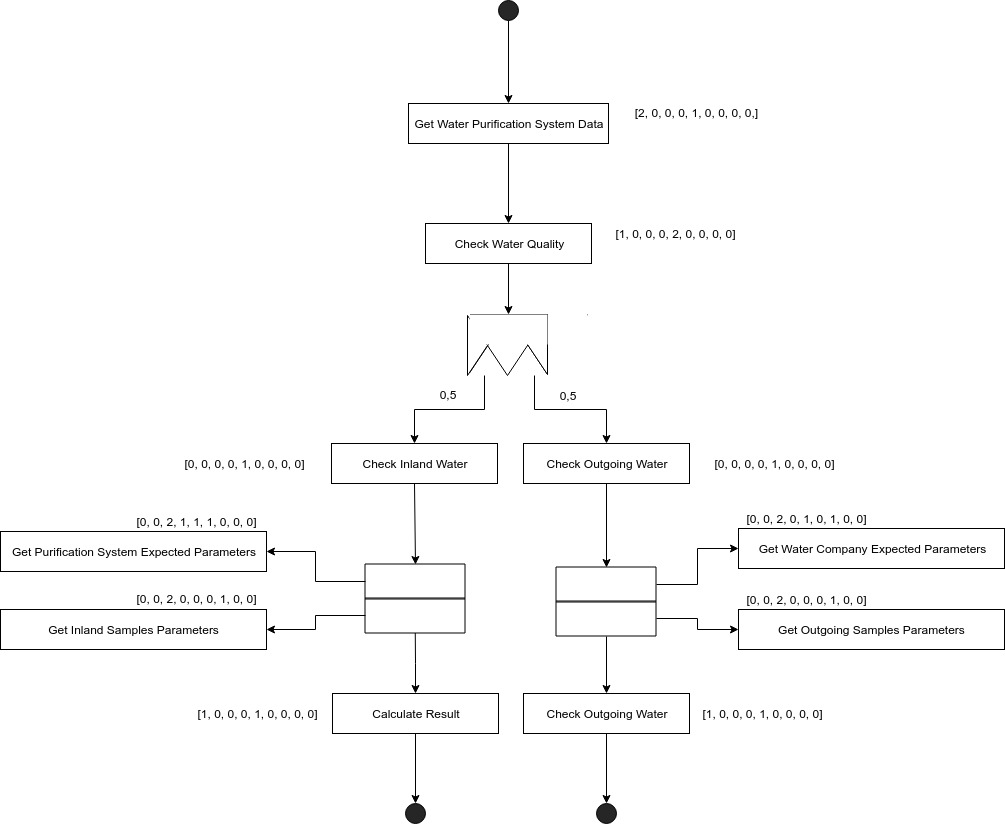
\includegraphics[width=\textwidth]				{EGUC3CheckWaterQuality.jpg}}
	\end{center}
	\bigskip
	\captionof{figure}{EG UC3 Check Water Quality}
\end{itemize}



